% This work is licensed under the Creative Commons
% Attribution-NonCommercial-ShareAlike 4.0 International License. To view a copy
% of this license, visit http://creativecommons.org/licenses/by-nc-sa/4.0/ or
% send a letter to Creative Commons, PO Box 1866, Mountain View, CA 94042, USA.

\section{Aufgabenblatt 8}

\subsection*{Aufgabe $\ast$)}
\begin{itemize}
	\item Transitionssystem ist $\A=(Q,\Sigma,I,\Delta,F)$ wobei
	\begin{itemize}
		\item $Q$ eine Menge von Zuständen ist (nicht notwendigerweise endlich!)
		\item $\Sigma$ ein endliches Alphabet
		\item $I\subseteq Q$ eine Menge von Anfangszuständen
		\item $\Delta\subseteq Q\times\Sigma\times Q$ eine Übergangsrelation (Transitionsrelation) ist
		\item $F\subseteq Q$ eine Menge von Endzuständen ist
	\end{itemize}
	\item Ein NEA ist ein Transitionssystem mit $|Q|<\infty$ und $|I|=1$.
	\item Ein NEA mit Wortübergängen hat die Form $\A=(Q,\Sigma,q_0,\Delta,F)$, wobei $Q,\Sigma,q_0,F$ wie beim NEA definiert sind und $\Delta\subseteq Q\times \Sigma^\ast\times Q$ eine endliche Menge von Wortübergängen ist. 
	(Beachte $\Sigma^\ast$!, somit ein NEA mit Wortübergängen \underline{kein} NEA!)
	\item Ein $\varepsilon$-NEA ist ein NEA mit Wortübergängen mit
	\begin{align*}
		\underbrace{|w|\leq1}_{\gdw w\in\Sigma\cup\lbrace\varepsilon\rbrace}\qquad\forall(q,w,q')\in\Delta
	\end{align*}
	\item $\varepsilon$-Übergang ist v.d.F. $(q,\varepsilon,q')\in Q\times\Sigma^\ast\times Q$
	\item Eine Menge $L$ von Wörtern mit $L\subseteq\Sigma^\ast$ heißt formale Sprache über $\Sigma$.
	\item unendliche Menge endlicher Wörter ist die Menge aller Wörter (= endliche Zeichenfolge) über $\Sigma$, i.Z. $\Sigma^\ast$.
\end{itemize}

\subsection*{Aufgabe $\ast\ast$)}
Für $L_1$ betrachte den NEA: $\A_1=(Q=\lbrace q_0,q_1,q_2\rbrace,\Sigma=\lbrace a,b\rbrace,q_0,\Delta,\lbrace q_2\rbrace)$ mit
\begin{align*}
	\Delta=\lbrace (q_0,a,q_1),(q_1,a,q_1),(q_1,b,q_1),(q_1,a,q_2)\rbrace\subseteq Q\times\Sigma\times Q
\end{align*}

\usetikzlibrary{positioning,automata}
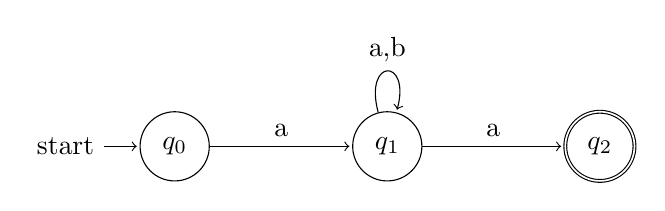
\begin{tikzpicture}[shorten >=1pt,node distance=2.7cm,on grid]
  \node[state,initial]   (q_0)                {$q_0$};
  \node[state]           (q_1) [right=of q_0] {$q_1$};
  \node[state,accepting] (q_2) [right=of q_1] {$q_2$};
  \path[->] (q_0) edge                node [above] {a} (q_1)
            (q_1) edge [loop above]   node [above] {a,b} ()
                  edge                node [above] {a} (q_2);
\end{tikzpicture}

Für $L_2$ betrachte den NEA: $\A_2=(Q=\lbrace q_0,q_1,q_2\rbrace,\Sigma=\lbrace a,b\rbrace,q_0,\Delta,\lbrace q_0\rbrace)$ mit $\Delta$ wie im Bild:

\usetikzlibrary{positioning,automata}
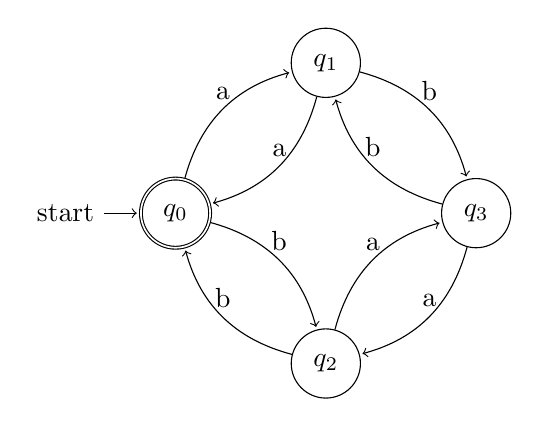
\begin{tikzpicture}[shorten >=1pt,node distance=2.7cm,on grid]
  \node[state,initial, accepting]   (q_0)                {$q_0$};
  \node[state]           (q_1) [above right=of q_0] {$q_1$};
  \node[state] (q_2) [below right=of q_0] {$q_2$};
  \node[state] (q_3) [above right=of q_2] {$q_3$};
  \path[->] (q_0) edge [bend left=30] node [above] {a} (q_1)
                  edge [bend left=30] node [above] {b} (q_2)
            (q_1) edge [bend left=30] node [above] {a} (q_0)
            	  edge [bend left=30] node [above] {b} (q_3)
            (q_2) edge [bend left=30] node [above] {b} (q_0)
                  edge [bend left=30] node [above] {a} (q_3)
            (q_3) edge [bend left=30] node [above] {b} (q_1)
                  edge [bend left=30] node [above] {a} (q_2);
\end{tikzpicture}


\subsection{Aufgabe 1}
\begin{align*}
	V_0:=\lbrace v_0\rbrace,\qquad V_{i+1}:=V_i\cup\big\lbrace v\in V\mid\exists v'\in V_i:(v',v)\in E\big\rbrace
\end{align*}

\begin{proof}
	Teil 1 Ist trivial nach Konstruktion (ansonsten kann man das leicht induktiv zeigen)\nl
	\ul{Zu Teil 2:}\\
	Die Folge $(V_i)_{i\in\N}$ ist nach Teil 1 monoton wachsend und durch die endliche (!) Menge $V$ nach oben beschränkt. 
	Folglich muss es einen Index geben, ab dem die Folge stationär wird.\nl
	Alternativ: Beweis durch Widerspruch: Angenommen, $V_i\neq V_{i+1}~\forall i\in\N$. 
	Aus Teil 1 folgt dann $V_i\varsubsetneqq V_{i+1}~\forall i\in\N.$ 
	Man sieht leicht, dass $V_i\subseteq V~\forall i\in\N$. 
	Damit existiert eine injektive Abbildung, welche jeder natürlichen Zahl $n\in\N$ ein Element aus $V_{n+1}\setminus V_n$ zuweist. 
	Damit gilt: $|\N|\leq |V|$. Dies ist ein Widerspruch zur Annahme, dass $V$ endlich ist.\nl
	Aufwand: $\mathcal{O}(|V|^2)$ %bin mir nicht ganz sicher
\end{proof}

\subsection{Aufgabe 2}
Ein DEA ist ein NEA, falls
\begin{align*}
	:\Longleftrightarrow\forall q\in Q,\forall a\in\Sigma:\exists!~q'\in Q:(q,a,q')\in\Delta
\end{align*}
Es erscheint sinnvoll, sich stets zuerst den NEA zu überlegen und danach diesen in einen DEA umzuschreiben.

\subsubsection{Aufgabe 2 a)}
\begin{align*}
	L_1=\big\lbrace a^n bac^m\mid m,n>0\text{ $n$ ist gerade und $m$ ist ungerade}\big\rbrace
\end{align*}
Wir konstruieren zuerst einen NEA, der $L_a$ akzeptiert:

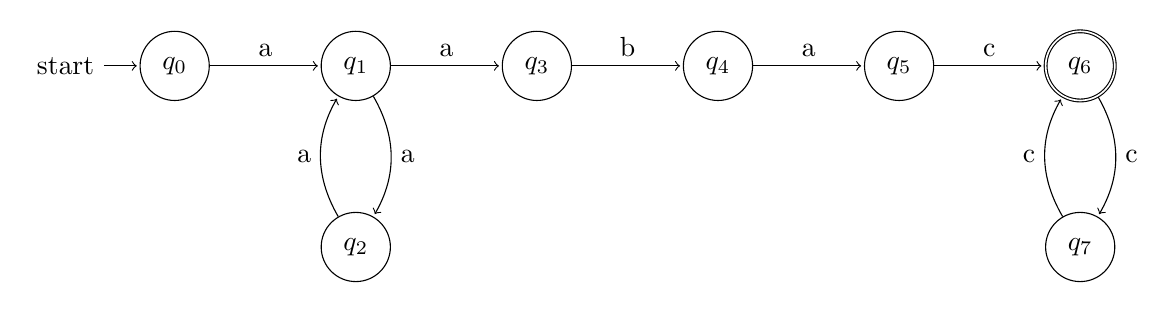
\begin{tikzpicture}[shorten >=1pt,node distance=2.3cm,on grid]
  \node[state,initial]   (q_0)                {$q_0$};
  \node[state]           (q_1) [right=of q_0] {$q_1$};
  \node[state]           (q_2) [below=of q_1] {$q_2$};
  \node[state]           (q_3) [right=of q_1] {$q_3$};
  \node[state]           (q_4) [right=of q_3] {$q_4$};
  \node[state]           (q_5) [right=of q_4] {$q_5$};
  \node[state, accepting](q_6) [right=of q_5] {$q_6$};
  \node[state]           (q_7) [below=of q_6] {$q_7$};
  \path[->] (q_0) edge                node [above] {a} (q_1)
            (q_1) edge                node [above] {a} (q_3)
                  edge [bend left=30] node [right] {a} (q_2)
            (q_2) edge [bend left=30] node [left]  {a} (q_1)
            (q_3) edge                node [above] {b} (q_4)
            (q_4) edge                node [above] {a} (q_5)
            (q_5) edge                node [above] {c} (q_6)
            (q_6) edge [bend left=30] node [right] {c} (q_7)
            (q_7) edge [bend left=30] node [left]  {c} (q_6);
\end{tikzpicture}

Um daraus einen DEA zu machen müssen wir:
\begin{itemize}
	\item Papierkorbzustände ergänzen
	\item Potenzmengenkonstruktion
\end{itemize}

Hier nun die Lösung aus der Übung (der Tutor stellte direkt den DEA auf und ging nicht obigen Umweg):

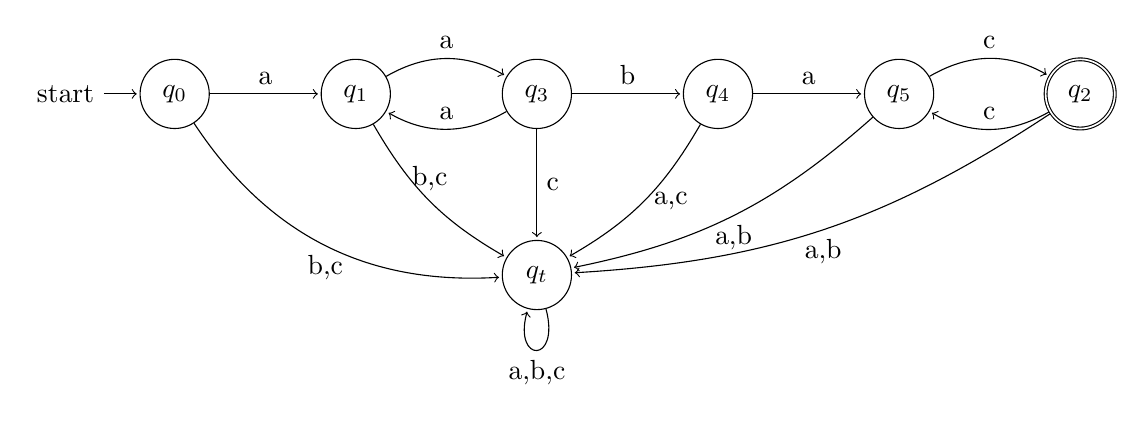
\begin{tikzpicture}[shorten >=1pt,node distance=2.3cm,on grid]
  \node[state,initial]   (q_0)                {$q_0$};
  \node[state]           (q_1) [right=of q_0] {$q_1$};
  \node[state]           (q_3) [right=of q_1] {$q_3$};
  \node[state]           (q_4) [right=of q_3] {$q_4$};
  \node[state]           (q_5) [right=of q_4] {$q_5$};
  \node[state, accepting](q_6) [right=of q_5] {$q_2$};
  \node[state]           (q_t) [below=of q_3] {$q_t$};
  \path[->] (q_0) edge                node [above] {a} (q_1)
                  edge [bend right=30] node [below] {b,c} (q_t)
            (q_1) edge [bend left=30] node [above] {a} (q_3)
                  edge [bend right=15]node [above] {b,c} (q_t)
            (q_3) edge                node [above] {b} (q_4)
                  edge [bend left=30] node [above] {a} (q_1)
                  edge                node [right] {c} (q_t)
            (q_4) edge                node [above] {a} (q_5)
                  edge [bend left=15] node [right] {a,c} (q_t)
            (q_5) edge [bend left=30] node [above] {c} (q_6)
                  edge [bend left=15] node [below] {a,b} (q_t)
            (q_6) edge [bend left=30] node [above] {c} (q_5)
                  edge [bend left=15] node [below] {a,b} (q_t)
            (q_t) edge [loop below]   node [below] {a,b,c} ();
\end{tikzpicture}

\subsubsection{Aufgabe b)}
\begin{align*}
	L_2=\big\lbrace w\in\lbrace0,1\rbrace^\ast\mid\exists i\in\lbrace0,1\rbrace:w\text{ endet mit $i$ \& enthält eine ungerade Anzahl $i$'s}\big\rbrace
\end{align*}

Konstruiere zuerst Automaten, welche Wörter über $\Sigma=\lbrace 0,1\rbrace$ erkennen, die mit $i$ enden und eine gerade Anzahl an $i$'s enthalten (für $i\in\lbrace0,1\rbrace$. 
Dann ``vereinige'' diese beiden Automaten in $\varepsilon$-NEA: 

\usetikzlibrary{positioning,automata}
\begin{minipage}[t]{0.49\textwidth}
	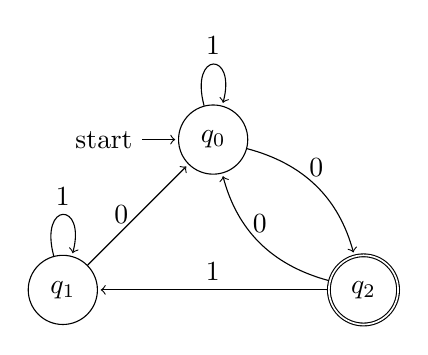
\begin{tikzpicture}[shorten >=1pt,node distance=2.7cm,on grid]
  \node[state,initial]   (q_0)                {$q_0$};
  \node[state]           (q_1) [below left=of q_0] {$q_1$};
  \node[state,accepting] (q_2) [below right=of q_0] {$q_2$};
  \path[->] (q_0) edge [bend left=30] node [above] {0} (q_2)
                  edge [loop above]   node [above] {1} ()
            (q_1) edge                node [left] {0} (q_0)
                  edge [loop above]   node [above] {1} ()
            (q_2) edge                node [above] {1} (q_1)
                  edge [bend left=30] node [above] {0} (q_0);
	\end{tikzpicture}
\end{minipage}
\begin{minipage}[t]{0.49\textwidth}
	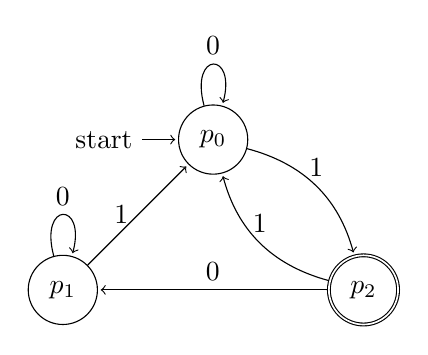
\begin{tikzpicture}[shorten >=1pt,node distance=2.7cm,on grid]
  \node[state,initial]   (p_0)                {$p_0$};
  \node[state]           (p_1) [below left=of p_0] {$p_1$};
  \node[state,accepting] (p_2) [below right=of p_0] {$p_2$};
  \path[->] (p_0) edge [bend left=30] node [above] {1} (p_2)
                  edge [loop above]   node [above] {0} ()
            (p_1) edge                node [left] {1} (p_0)
                  edge [loop above]   node [above] {0} ()
            (p_2) edge                node [above] {0} (p_1)
                  edge [bend left=30] node [above] {1} (p_0);
	\end{tikzpicture}
\end{minipage}

Vereinigen liefert:

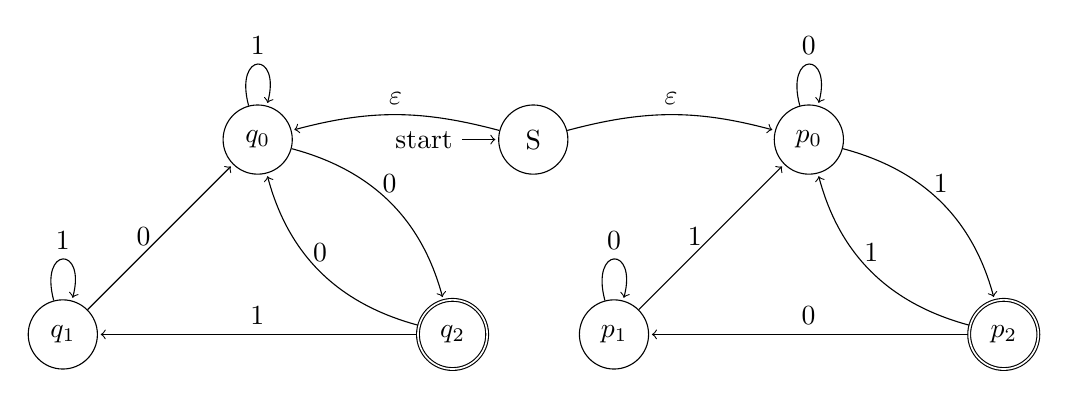
\begin{tikzpicture}[shorten >=1pt,node distance=3.5cm,on grid]
  \node[state,initial]   (S)                       {S};
  \node[state]           (q_0) [left=of S]   {$q_0$};
  \node[state]           (q_1) [below left=of q_0] {$q_1$};
  \node[state,accepting] (q_2) [below right=of q_0]{$q_2$};
  \node[state]           (p_0) [right=of S]  {$p_0$};
  \node[state]           (p_1) [below left=of p_0] {$p_1$};
  \node[state,accepting] (p_2) [below right=of p_0]{$p_2$};
  \path[->] (S)   edge [bend right=15] node [above] {$\varepsilon$} (q_0)
                  %edge                node [above] {0} (q_2)
                  edge [bend left=15] node [above] {$\varepsilon$} (p_0)
                  %edge                node [below right] {1} (p_2)
            (q_0) edge [bend left=30] node [above] {0} (q_2)
                  edge [loop above]   node [above] {1} ()
            (q_1) edge                node [left] {0} (q_0)
                  edge [loop above]   node [above] {1} ()
            (q_2) edge                node [above] {1} (q_1)
                  edge [bend left=30] node [above] {0} (q_0)
            (p_0) edge [bend left=30] node [above] {1} (p_2)
                  edge [loop above]   node [above] {0} ()
            (p_1) edge                node [left] {1} (p_0)
                  edge [loop above]   node [above] {0} ()
            (p_2) edge                node [above] {0} (p_1)
                  edge [bend left=30] node [above] {1} (p_0);
\end{tikzpicture}

Wir haben nun einen $\varepsilon$-NEA. 
Nun entfernen wir die $\varepsilon$-Transitionen:

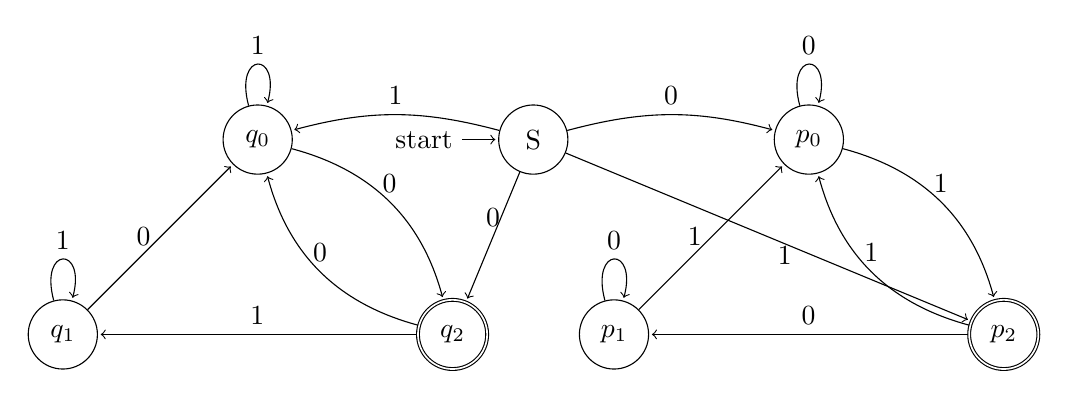
\begin{tikzpicture}[shorten >=1pt,node distance=3.5cm,on grid]
  \node[state,initial]   (S)                       {S};
  \node[state]           (q_0) [left=of S]   {$q_0$};
  \node[state]           (q_1) [below left=of q_0] {$q_1$};
  \node[state,accepting] (q_2) [below right=of q_0]{$q_2$};
  \node[state]           (p_0) [right=of S]  {$p_0$};
  \node[state]           (p_1) [below left=of p_0] {$p_1$};
  \node[state,accepting] (p_2) [below right=of p_0]{$p_2$};
  \path[->] (S)   edge [bend right=15] node [above] {1} (q_0)
                  edge                node [above] {0} (q_2)
                  edge [bend left=15] node [above] {0} (p_0)
                  edge                node [below right] {1} (p_2)
            (q_0) edge [bend left=30] node [above] {0} (q_2)
                  edge [loop above]   node [above] {1} ()
            (q_1) edge                node [left] {0} (q_0)
                  edge [loop above]   node [above] {1} ()
            (q_2) edge                node [above] {1} (q_1)
                  edge [bend left=30] node [above] {0} (q_0)
            (p_0) edge [bend left=30] node [above] {1} (p_2)
                  edge [loop above]   node [above] {0} ()
            (p_1) edge                node [left] {1} (p_0)
                  edge [loop above]   node [above] {0} ()
            (p_2) edge                node [above] {0} (p_1)
                  edge [bend left=30] node [above] {1} (p_0);
\end{tikzpicture}

Jetzt nutzen wir die Potenzmengenkonstruktion, um daraus einen DEA zu erhalten. Dabei gehen wir \textit{On-the-fly} vor:
\begin{itemize}
	\item Betrachte zuerst die Menge der Knoten, die man vom Startzustand aus über Kante $i$ erreicht.
	\item Eine solche Menge wird Endzustand gdw. ein Element davon Endzustand war.
\end{itemize}

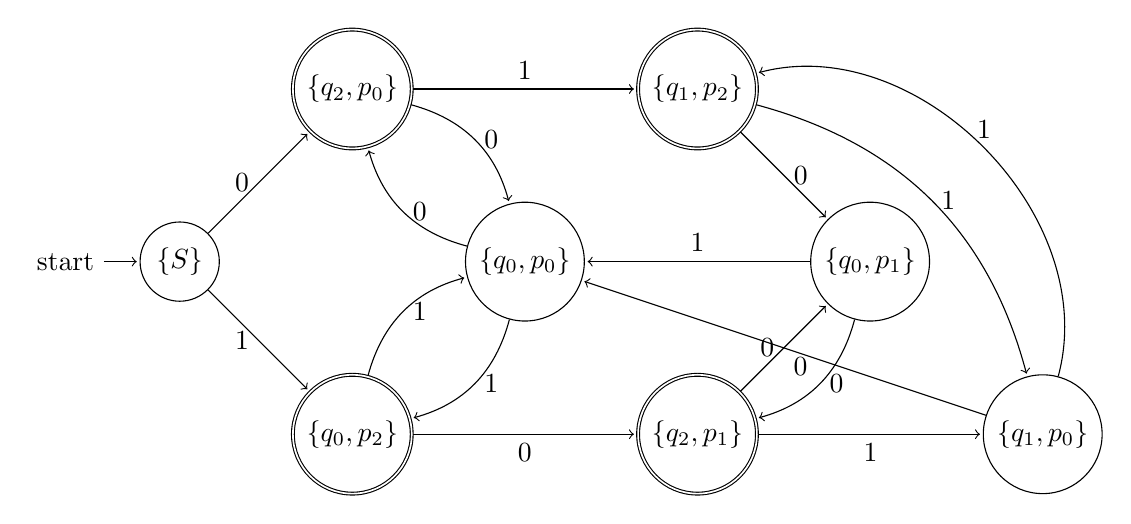
\begin{tikzpicture}[shorten >=1pt,node distance=3.1cm,on grid]
  \node[state,initial]   (S)                       {$\lbrace S\rbrace$};
  \node[state,accepting] (q_2p_0) [above right=of S]   {$\lbrace q_2,p_0\rbrace$};
  \node[state, accepting](q_0p_2) [below right=of S] {$\lbrace q_0,p_2\rbrace$};
  \node[state]           (q_0p_0) [below right=of q_2p_0]{$\lbrace q_0,p_0\rbrace$};
  \node[state,accepting] (q_1p_2) [above right=of q_0p_0] {$\lbrace q_1,p_2\rbrace$};
  \node[state,accepting] (q_2p_1) [below right=of q_0p_0] {$\lbrace q_2,p_1\rbrace$};
  \node[state]           (q_0p_1) [below right=of q_1p_2]{$\lbrace q_0,p_1\rbrace$};
  \node[state]           (q_1p_0) [below right=of q_0p_1]{$\lbrace q_1,p_0\rbrace$};
  \path[->] (S)   edge [bend right=0] node [left] {0} (q_2p_0)
                  edge [bend right=0] node [left] {1} (q_0p_2)
         (q_2p_0) edge [bend right=0] node [above]{1} (q_1p_2)
                  edge [bend left=30] node [right]{0} (q_0p_0)
         (q_0p_2) edge [bend right=0] node [below]{0} (q_2p_1)
                  edge [bend left=30] node [right]{1} (q_0p_0)
         (q_0p_0) edge [bend left=30] node [right]{0} (q_2p_0)
         		  edge [bend left=30] node [right]{1} (q_0p_2)
         (q_1p_2) edge [bend right=0] node [right]{0} (q_0p_1)
                  edge [bend left=30] node [right]{1} (q_1p_0)
         (q_2p_1) edge [bend right=0] node [below]{1} (q_1p_0)
                  edge [bend right=0] node [left]{0} (q_0p_1)
         (q_0p_1) edge [bend left=30] node [right]{0} (q_2p_1)
         		  edge [bend right=0] node [above]{1} (q_0p_0)
		 (q_1p_0) edge [bend left=300]node [above]{1} (q_1p_2)
		          edge [bend left=0] node [below right]{0} (q_0p_0)         
         ;
\end{tikzpicture}

\subsection{Aufgabe 3}
Zwei Transitionssysteme (NEAs sind Spezialfälle) heißen \textbf{äquivalent}, wenn sie dieselbe Sprache akzeptieren.\\
Formaler: Seien $\A=(Q,\Sigma,q_0,\Delta,F),\A'=(Q',\Sigma',q_0',\Delta',F')$ zwei NEAs. 
Diese sind äquivalent
\begin{align*}
	&\Longleftrightarrow L(\A_1)=L(\A_2)\\
	&\Longleftrightarrow \big\lbrace w\in\Sigma^\ast:\A_1\text{ akzeptiert }w\big\rbrace
	=\big\lbrace w\in\Sigma'^\ast:\A_2\text{ akzeptiert }w\big\rbrace\\
	&\Longleftrightarrow\big\lbrace w\in\Sigma^\ast:I\stackrel{w}{\longrightarrow}_{\A_1} F\big\rbrace=
	\big\lbrace w\in\Sigma'^\ast:I'\stackrel{w}{\longrightarrow}_{\A_2} F'\big\rbrace
\end{align*}

Wir erhalten die Lösung mithilfe der Potenzmengenkonstruktion:

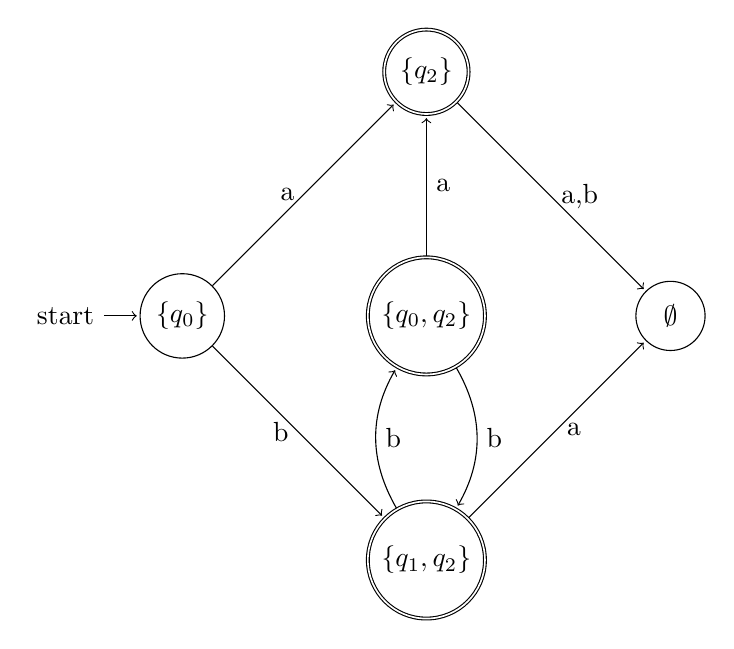
\begin{tikzpicture}[shorten >=1pt,node distance=3.1cm,on grid]
  \node[state,initial]   (q_0)                       {$\lbrace q_0\rbrace$};
  \node[state,accepting] (q_0q_2) [right = of q_0]   {$\lbrace q_0,q_2\rbrace$};
  \node[state,accepting] (q_2) [above=of q_0q_2]        {$\lbrace q_2\rbrace$};
  \node[state,accepting] (q_1q_2) [below=of q_0q_2] {$\lbrace q_1,q_2\rbrace$};
  \node[state]           (t)      [right = of q_0q_2] {$\emptyset$};
  \path[->] (q_0) edge [bend right=0] node [left] {a} (q_2)
                  edge [bend right=0] node [left] {b} (q_1q_2)
         (q_2)    edge [bend right=0] node [right]{a,b} (t)
         (q_0q_2) edge [bend right=0] node [right]{a} (q_2)
                  edge [bend left=30] node [right]{b} (q_1q_2)
         (q_1q_2) edge [bend left=0]  node [right]{a} (t)
         		  edge [bend left=30] node [right]{b} (q_0q_2)     
         ;
\end{tikzpicture}

\subsection{Aufgabe 4}
Sei $\A=(Q,\Sigma,I,\delta,F)$ ein DEA.

\subsubsection{Aufgabe 4 a)}
\begin{align*}
	\forall\lbrace u,v\rbrace\subseteq\Sigma^\ast,\forall q\in Q:\delta(q,uv)=\delta\big(\delta(q,u),v\big)
\end{align*}

\begin{proof}
	Beweis durch Induktion über die Länge von $v$ beliebigem $u\in\Sigma^\ast$.\\
	Erinnerung an die Definition:
	\begin{align}
		\delta^\ast(q,\varepsilon)&:=q\label{eq1}\\
		\delta^\ast(q,wa)&:=\delta\big(\delta^\ast(q,w),a\big)\label{eq2}
	\end{align}
	\ul{IA:} $|v|=0$, d.h. $v=\varepsilon$:
	\begin{align*}
		\delta^\ast(q,uv)\overset{u\cdot\varepsilon=u}&{=}
		\delta^\ast(q,u)
		\overset{\eqref{eq1}}{=}
		\delta^\ast\big(\delta^\ast(q,u),\varepsilon\big)
		=\delta^\ast\big(\delta^\ast(q,u),v\big)
	\end{align*}
	\ul{IH:} Für alle $v\in\Sigma^n$ gilt: $\delta^\ast(q,uv)=\delta^\ast\big(\delta^\ast(q,u),v\big)$\nl
	\ul{IS:} Sei $v'\in\Sigma^{n+1}$, d.h. es existiert $v\in\Sigma^n$ und $a\in\Sigma$ mit $v'=va$.
	\begin{align*}
		\delta^\ast\big(q,uv'\big)
		&=
		\delta^\ast\big(q,uva\big)\\
		\overset{\eqref{eq2}}&=
		\delta\big(\delta^\ast(q,uv),a\big)\\
		\overset{\text{IH}}&=
		\delta\big(\delta^\ast\big(\delta^\ast(q,u),v\big),a\big)\\
		\overset{\eqref{eq2}}&=
		\delta^\ast\big(\delta^\ast(q,u),va\big)\\
		&=
		\delta^\ast\big(\delta^\ast(q,u),v'\big)
	\end{align*}
\end{proof}

\subsubsection{Aufgabe 4 b)}
\begin{align*}
	\sim_k=\sim_{k+1}\implies\sim_k=\sim_\A
\end{align*}

\begin{proof}
	Angenommen es gilt $\sim_k=\sim_{k+1}$ für ein festes $k\in\N$. 
	Dann gilt:
	%TODO
\end{proof}
